\documentclass{beamer}
\usepackage[english]{babel}
\usepackage[utf8]{inputenc}
\usepackage[T1]{fontenc}

\usepackage{bm}
%\usepackage{math}
\usepackage{physics}

\usepackage{pgfplots}
% and optionally (as of Pgfplots 1.3):
\pgfplotsset{compat=newest}
\pgfplotsset{plot coordinates/math parser=false}
\newlength\figureheight
\newlength\figurewidth
\usepackage{environ}

\newcommand{\Hilbert}{\mathcal{H}}
\newcommand{\Vector}[1]{\bm{\MakeLowercase{#1}}}
\newcommand{\Operator}[1]{\bm{\MakeUppercase{#1}}}
%%%%%%%%%%
\DeclareMathAlphabet{\mathsfbr}{OT1}{cmss}{m}{n}%for math sans serif (cmss)
\SetMathAlphabet{\mathsfbr}{bold}{OT1}{cmss}{bx}{n}%for math sans serif (cmss)
\DeclareRobustCommand{\msf}[1]{%
  \ifcat\noexpand#1\relax\msfgreek{#1}\else\mathsfbr{#1}\fi%for math sans serif (cmss)
}
\DeclareFontEncoding{LGR}{}{} % or load \usepackage{textgreek}
\DeclareSymbolFont{sfgreek}{LGR}{cmss}{m}{n}
\SetSymbolFont{sfgreek}{bold}{LGR}{cmss}{bx}{n}
\DeclareMathSymbol{\sXi}{\mathalpha}{sfgreek}{`X}
\DeclareMathSymbol{\sUpsilon}{\mathalpha}{sfgreek}{`U}
%%%%%%%%%%

%\usetheme[titlepagelogo=Pictures/logo.png,
%          language=english,
%          bullet=square,
%          color=blue,
%          coding=utf8, % occhio solo a questo, se non funziona usa pure latin1
%          secondsupervisor=false,
%          assistantsupervisor=true,
%         ]{TorinoTh}

\usetheme{Ferrara}

\author[Federico Forzano]{
                        {\scriptsize Supervisor:}\hspace{60mm}{\scriptsize Candidate:}\\
                        Chiar.mo~Prof.~Andrea Conti \hspace{25mm} Federico Forzano\\
                        {\scriptsize Co-Supervisor:}\\
                        Dott.~Ing.~Stefano Guerrini
                        }

\title{On the Design of Quantum Communication Systems with non-Gaussian States}

\date{}

\begin{document}
        
    
    \input{Frame/TitleFrame.tex}

    % Capitolo 1: Quantum Mechanics Abstract
    %\begin{frame}
    \frametitle{Quantum Mechanics Abstract}
    \framesubtitle{Postulates}

    \begin{block}{Postulate 1: State Representation}
        The state of an isolated quantum system is represented by a complex unitary 
        vector in an Hilbert space:
        \begin{equation*}
            \ket{\psi} \in \Hilbert
        \end{equation*}
    \end{block}
    %
    \begin{block}{Postulate 2: Observables}
        Every observables of the system is represented by an Hermitian operator
        acting on the state space:
        \begin{equation*}
            \mathcal{M}:\Hilbert\to\Hilbert
        \end{equation*}
    \end{block}
\end{frame}

\begin{frame}
    \frametitle{Quantum Mechanics Abstract}
    \framesubtitle{Postulates}

    \begin{block}{Postulate 3: Born's Rule}
        The probability to get the measurement $\lambda_i$ from the observable 
        $\mathcal{M}$ in the system in state $\ket{\psi}$ is:
        \begin{equation*}
            %\mathbb{P}(\lambda_i)=\braket{\psi}{\lambda_i}\braket{\lambda_i}{\psi}
            \mathbb{P}(\lambda_i)=\bra{\psi}\mathcal{P}_i\ket{\psi}
        \end{equation*}
    \end{block}
    %
    \begin{block}{Postulate 4: Wavefunction Collapse}
        The state after measurement of $\lambda_i$ is $\mathcal{P}_i\ket{\psi}$ (with the
        necessary normalization):
        \begin{equation*}
            \ket{\psi'}=\frac{\mathcal{P}_i\ket{\psi}}{\bra{\psi}\mathcal{P}_i\ket{\psi}}.
        \end{equation*}
    \end{block}
\end{frame}

\begin{frame}
    \frametitle{Quantum Mechanics Abstract}
    \framesubtitle{Postulates}

    \begin{block}{Postulate 5: Time Evolution}
        The time evolution of an isolated quantum system is given by an unitary operator
        $\mathcal{U}$:
        \begin{equation*}
            \ket{\psi(t)}=\mathcal{U}(t_0,t)\ket{\psi(t_0)}.
        \end{equation*}
    \end{block}
    %
    \begin{block}{Postulate 6: Composite System}
        The state space of a system composed of $\Hilbert_1$ and $\Hilbert_2$ is given by
        \begin{equation*}
            \Hilbert=\Hilbert_1\otimes\Hilbert_2.
        \end{equation*}
    \end{block}

\end{frame}
    %\section{Quantized Electromagnetic Field}
    Electromagnetic field is the main means of communication for contemporary
    application. It is important therefor, to give a quantum representation.
    In this section the representation of quantized electromagnetic field is 
    initially given, so the Fock representation of a state is introduced.
            
    \subsection{Classical electromagnetic field}
        In a volume $\mathcal{V}\in\mathbb{R}^3$ classical electromagnetic field is 
        determinated from Maxwell's equations as a superposition of the cavity modes
        (\cite{tesiGuerrini} quoting \cite{quantumRad_Louissel,quantumOptic_Mandel}).
        Electric field is given by the well-known expression:
        \begin{equation}
            \pmb{e}(\pmb{r},t)=\sum_n p_n (t)\pmb{u}_n (\pmb{r})
            \label{eq:CEF.1}
        \end{equation}
        where
        \begin{equation*}
            \pmb{u}_n (\pmb{r})=\pmb{u}_{n0}\ e^{i\pmb{k}_n \cdot \pmb{r}}
        \end{equation*}
        and $\pmb{u}_{n0}$ is determinated by the initial condition.
        The corresponding magnetic field is determinated by:
        \begin{equation}
            \pmb{h}(\pmb{r},t)=\sum_n q_n (t)\nabla\times\pmb{u}_n (\pmb{r})
            \label{eq:CEF.2}
        \end{equation}
        and
        \begin{equation}
            p_n (t)=\derivative{q_n (t)}{t} .
            \label{eq:CEF.3}
        \end{equation}
        The Hemiltonian associated to the n-th mode is given by
        \begin{equation}
            H_n=\frac{1}{2}[p_n^2(t)+\omega_n^2q_n^2(t)].
            \label{eq:CEF.4}
        \end{equation}
        Equivalently, it is possible to define the complex variable $a_n(t)$ as
        \begin{equation}
            a_n(t)=\frac{\omega_nq_n(t)+ip_n(t)}{\sqrt{2\hbar\omega_n}}
            \label{eq:CEF.5}
        \end{equation}
        and, using \ref{eq:CEF.5} in \ref{eq:CEF.4}, it is possible to obtain the following
        expression of the Hemiltonian:
        \begin{equation}
            H_n=\hbar\omega_n\absolutevalue{a_n(t)}^2.
            \label{eq_CEF.6}
        \end{equation}

    \subsection{Quantized electromagnetic field}
        The quantization of electromagnetic field is obtained replacing the two quantities 
        $p_n(t)$ and $q_n(t)$ with the Hermitian operators 
        $\pmb{P}_n(t),\ \pmb{Q}_n(t):\Hilbert_n\to\Hilbert_n$ and by imposing the following
        commutation conditions (\cite{tesiGuerrini} quoting \cite{quantumRad_Louissel,quantumOptic_Mandel}):
        \begin{equation}
            \commutator{\pmb{Q}_n}{\pmb{P}_m}=i\hbar\delta_{n,m}\pmb{I}
        \end{equation}
        \begin{equation}
            \commutator{\pmb{Q}_n}{\pmb{Q}_m}=0
        \end{equation}
        \begin{equation}
            \commutator{\pmb{P}_n}{\pmb{P}_m}=0.
        \end{equation}
        Defining the annihilation operator $\pmb{A}_n$ as
        \begin{equation}
            \pmb{A}_n(t)=\frac{\omega_n\pmb{Q}_n(t)+i\pmb{P}_n(t)}{\sqrt{2\hbar\omega_n}}
            \label{eq:QEF.1}
        \end{equation} 
        and the adjoint of $\pmb{A}_n$, the creation operator $\pmb{A}_n^\dagger$ as
        \begin{equation}
            \pmb{A}_n(t)=\frac{\omega_n\pmb{Q}_n(t)-i\pmb{P}_n(t)}{\sqrt{2\hbar\omega_n}}
            \label{eq:QEF.2}
        \end{equation}
        it is possible to describe the Hemiltonian of the system as
        \begin{equation}
            H_n=\hbar\omega_n\pmb{A}_n^\dagger\pmb{A}_n.
            \label{eq:QEF.3}
        \end{equation}

    \subsection{Fock states}
        In a single mode cavity, it is possible to define the number operator $\pmb{N}$ as
        \begin{equation}
            \pmb{N}=\pmb{A}^\dagger \pmb{A}.
        \end{equation}
        Single mode Fock states are the eigenvector of $N$, i.e the solution of equation:
        \begin{equation}
            \pmb{N}\ket{n}=n\ket{n}.
        \end{equation}
        The Fock state $\ket{n}$ represent the quantum state with exactly n photons.
        It is important to evidence that the set of all Fock states forms an orthonormal basis
        of the Hilbert space $\Hilbert$, so every state $\Xi$ can be expressed as
        \begin{equation}
            \pmb{\Xi} = \sum_{n,m} c_{n,m}\ket{n}\bra{m}
            \label{eq:QEF.4}
        \end{equation}
        with
        \begin{equation*}
            c_{n,m}=\bra{n}\pmb{\Xi}\ket{m}.
        \end{equation*}

        Using the representation in Fock basis, it is possible to charaterize some type of quantum 
        states of the quantum electromagnetic field. In the following section the states studied 
        are briefly described.
    %\begin{frame}
    \frametitle{Quantum Mechanics Abstract}
    \framesubtitle{Fock states}

    \begin{block}{Fock State}<1->
        The Fock state $\ket{n}$ represents the quantum state with exactly n photons. It is 
        defined as:
        \begin{equation*}
            \pmb{N}\ket{n}=n\ket{n}\ \ with\ \pmb{N}=\pmb{A}^\dagger \pmb{A}
        \end{equation*}
    \end{block}
    \begin{alertblock}{Fock Representation}<2->
        Every quantum state $\pmb{\Xi}$ can be expressed as
        \begin{equation*}
            \pmb{\Xi} = \sum_{n,m} c_{n,m}\ket{n}\bra{m}\ \ with\ c_{n,m}=\bra{n}\pmb{\Xi}\ket{m}
        \end{equation*}
    \end{alertblock}

\end{frame}
    %\begin{frame}{Quantum Mechanics Abstract}{Wigner W-Function}
    \begin{block}{s-order characteristic function}<1->
        \begin{equation*}
            \mathcal{\chi}(\xi,s)=\exp{\frac{s}{2}\absolutevalue{\xi}^2}
            tr\{\pmb{\Xi}\pmb{D}_\xi\}
        \end{equation*}
    
        \center{$\pmb{D}_\xi=\exp{\xi\pmb{A}^\dagger-\xi^*\pmb{A}}$ \ \  \emph{Displacement Operator}}
    \end{block}
    \begin{block}{s-order quasi-probability function}<2->
        \begin{equation*}
            W(\alpha,s)=\frac{1}{\pi^2}\int_{\mathbb{R}^2} 
            \mathcal{\chi}(\xi,s)e^{\alpha\xi^*-\alpha^*\xi}d\xi^2.
        \end{equation*}
        The quasi-probability function for $s=0$ is called Wigner W-function.
    \end{block}
    \ \\ \mbox{} \\
\end{frame}
    %\begin{frame}{Quantum Mechanics Abstract}{Wigner Function}

\end{frame}

    \section{Motivation}
    \begin{frame}{Motivation}
    \begin{itemize}
        \item Communications are becoming ever more important and widespread.
        \item Classical physics is only a special case of quantum physics.
        \item The use of quantum non-Gaussian states can significantly improve the performance 
                of a communication system.
    \end{itemize}
\end{frame}
    \begin{frame}{Contents}
        \tableofcontents
    \end{frame}

    % Capitolo 2: Quantum Communication
    \section{Quantum Communication System}
    \begin{frame}{Quantum Communication System}
    \includegraphics[width=1\textwidth]{Pictures/fig3.0.pdf}
    \begin{center}
        {\scriptsize 
        Block chain of a quantum communication system.
        }
    \end{center}
\end{frame}
    \subsection{Quantum modulator}
    \section{Quantum Modulation}
    As in a classical system, it is possible to define the concept of modulation for a 
    quantum communication system. The trasmitted information, will be associated to a 
    quantum state of the electromagnetic field, so it can be trasmitted on the communication 
    channel.

    \begin{figure}[ht]
        \includegraphics[width=1\textwidth]{fig2.1.pdf}
        \caption{Block diagram of a quantum trasmitter.}
        \label{fig:2.1}
    \end{figure}
    It is possible to think about the quantum trasmitter as in figure \ref{fig:2.1}. The bit source
    emits a bit sequence, the serial-parallel converter parallelize a group of $l$-bit (where, if $L$
    is the number of quantum states, $l=\log_2(L)$) and sends them to the quantum modulator; this last
    associate to every group of bit, one quantum state. The operation of quantum state creation, 
    in real cases, is affected by noise.

    The sequence of operation is very closer to a classical trasmitter, the main difference is that
    the modulator map the bits into quantum states instead of classical modulation. It is, therefor, 
    possible to achieve the equivalent of classical modulation, that it is called quantum modulation,
    with several states and assess the impact on performance.
    In this thesis only the binary will be considered and assessed, in the OOK and BPSK configuration.
    
    \subsection{OOK modulation}

    \subsection{BPSK modulation}

    \begin{frame}{Quantum Mechanics Abstract}{Wigner Function}

\end{frame}
    \subsection{Quantum receiver}
    \section{Quantum Discriminator}
    The problem of quantum state discrimination (QSD) are one of the most important
    aspect of quantum communication. As in classical communication, the ability to 
    distinguish between two or more states, in presence of noise, can be decisive for improve
    the performance of the communication system. Unlike the classical situation however,
    the discrimination can be done using a custom-designed quantum discriminator, overcoming
    the classical physics limits.

    \subsection{Binary quantum state discrimination}
    \begin{figure}[ht]
        \begin{center}
            \includegraphics[width=0.75\textwidth]{fig2.2.pdf}
            \caption{Binary quantum state discriminator.}
            \label{fig:2.2}
        \end{center}
    \end{figure}
    The problem of discrimination between two quantum states is realized, as every measurement
    process \ref{post:2}, using an operator or with a set of operators.
    If the state of system is unknown, as shown in figure \ref{fig:2.2}, there are two hypotheses
    about the state $\pmb{\Xi}$ (the problem is generalises easly for $M$ different states),
    given by:
    \begin{equation}\begin{split}
        H_0 : \pmb{\Xi}=\pmb{\Xi}_0\\
        H_1 : \pmb{\Xi}=\pmb{\Xi}_1
        \label{eq:binHyp}
    \end{split}\end{equation}
    It is necessary a set of two positive-definites operator (POVM):
    \begin{equation}
        \mathcal{P}=\{\pmb{\Pi}_0,\pmb{\Pi}_1\}
    \end{equation}
    for the discrimination process and the probability that the hypothesis $H_j$ is choosen
    if $H_k$ is the right choose, is given by \cite{tesiGuerrini}:
    \begin{equation}
        \mathbb{P}\{H_j|H_k\}=tr\{\pmb{\Xi}_k\pmb{\Pi}_j\}.
    \end{equation}
    The distribution error probability (DEP) in the discrimination process, if $p_0$ and $p_1$ are 
    respectively the probabilty of symbols $0$ and $1$, is so given by
    \begin{equation}
        P_e=1-\left(p_0 tr\{\pmb{\Xi}_0\pmb{\Pi}_0\}+p_1 tr\{\pmb{\Xi}_0\pmb{\Pi}_0\}\right).
    \end{equation}

    \subsection{Optimal discriminator}
    The issue of finding the optimal POVM that minimize was exhaustively discuss  by Helstrom in 
    \cite{helstrom3,helstrom4}. The minimum distribution error probability (MDEP), for a binary 
    communication system, is given by the well-known Helstrom bound
    \begin{equation}
        \breve{P}_e = \frac{1}{2} \left(1-\norm{p_1 \pmb{\Xi}_1 - p_0 \pmb{\Xi}_0}_1 \right),
        \label{eq:HelstromBound}
    \end{equation}
    where $p_0,\ p_1$ are the probability that the states $\pmb{\Xi}_0,\ \pmb{\Xi}_1$ are trasmitted
    and the operator $\norm{\cdot}_1$ represents the trace norm. 
    The MDEP \ref{eq:HelstromBound} is obtained with the following POVM:
    \begin{equation}
        \breve{\pmb{\Pi}}_0 = \sum_{\substack{i \\ \lambda_i<0}} \ket{\lambda_i}\bra{\lambda_i},
    \end{equation}
    \begin{equation*}
        \breve{\pmb{\Pi}}_1 = 1-\breve{\pmb{\Pi}}_0 = 
        \sum_{\substack{i \\ \lambda_i \geq 0}} \ket{\lambda_i}\bra{\lambda_i};
    \end{equation*}
    where $\ket{\lambda_i}$ is the eigenvector of $p_1 \pmb{\Xi}_1 - p_0 \pmb{\Xi}_0$ associated to 
    the eigenvalue $\lambda_i$.
    For pure states, i.e $\pmb{\Xi}_0 = \ket{\psi_0}\bra{\psi_0}$ and $\pmb{\Xi}_1 = \ket{\psi_1}
    \bra{\psi_1}$, the equation \ref{eq:HelstromBound} begin
    \begin{equation}
        \breve{P}_e = \frac{1}{2} \left(1- \sqrt{1-4 p_0 p_1 \absolutevalue{\braket{\psi_0}{\psi_1}}^2}
        \right).
    \end{equation}
    It is possible to observe that, for pure states, the MDEP is equal to $0$ if $\braket{\psi_0}{\psi_1}$,
    that is $\ket{\psi_0}$ and $\ket{\psi_1}$ are orthogonal states.

    % Capitolo 3: Discrimination of Photon Added States
    \section{Performance Analysys}
    \subsection{PACS system performance}
    %\begin{frame}{Discrimination of Photon Added States}{Noisy PACS discrimination: OOK}
%    \begin{center}
%        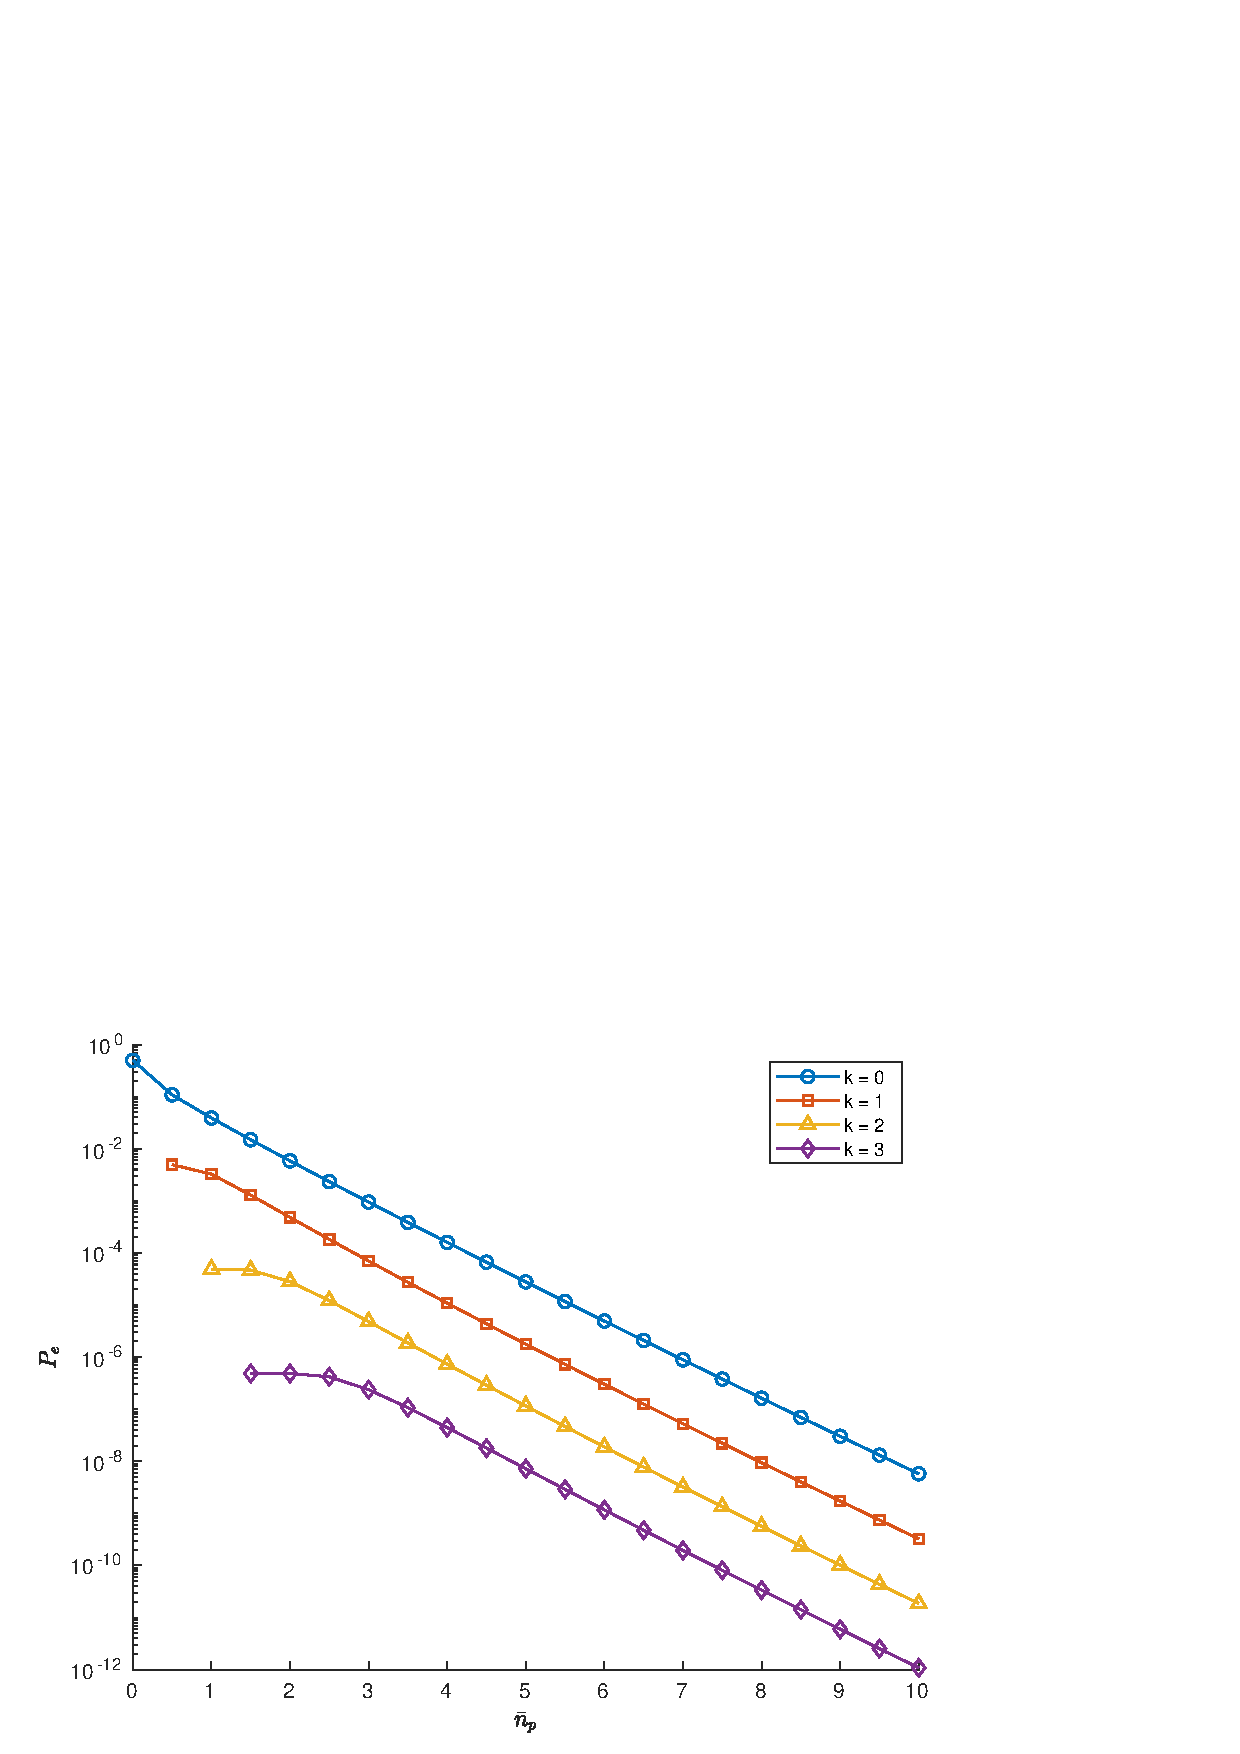
\includegraphics[width=0.65\textwidth]{Pictures/fig3.1.pdf}\\
%        \scriptsize{
%        MDEP of a QOOK system with PACS in terms of the mean photon number $n_p$.\\
%        $k=0,1,2,3$; $N=30$; $\bar{n}=10^{-2}$; $p_0=p_1=1/2$
%        }
%    \end{center}
%\end{frame}

\begin{frame}{Discrimination of Photon Added States}{Noisy PACS discrimination}
    \begin{center}
        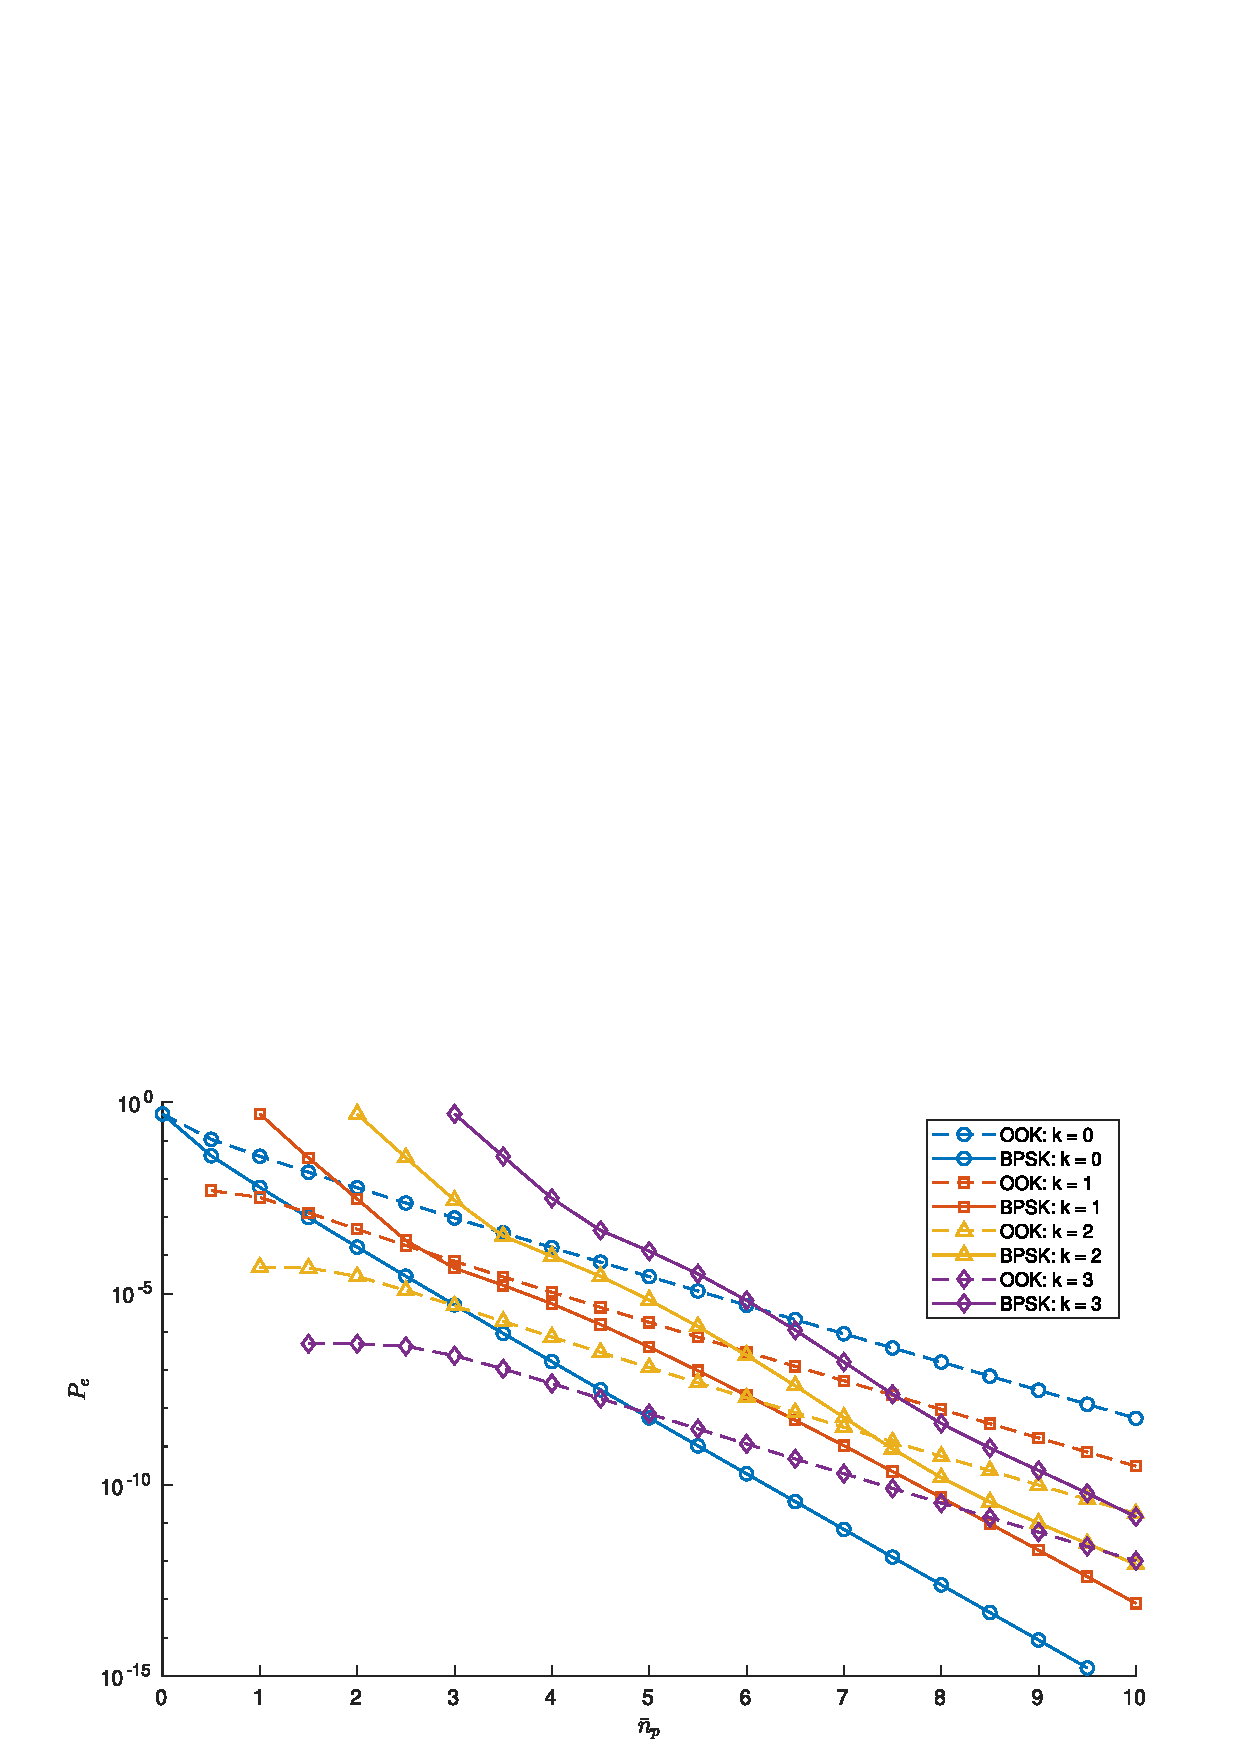
\includegraphics[width=1\textwidth]{Pictures/fig3.4.pdf}\\
        \scriptsize{
        MDEP comparison of a QOOK and QBPSK systems with PACS in terms of the mean energy of the system $\bar{E}$.\\
        $N=45$; $\bar{n}=10^{-2}$; $p_0=p_1=1/2$
        }
    \end{center}
    \ \mbox{}\\ \ \mbox{}\\
\end{frame}
    \subsection{Noise effect}
    \begin{frame}{Discrimination of Photon Added States}{Noise effect}
    \begin{columns}
        \begin{column}{0.5\linewidth}
            \begin{center}
                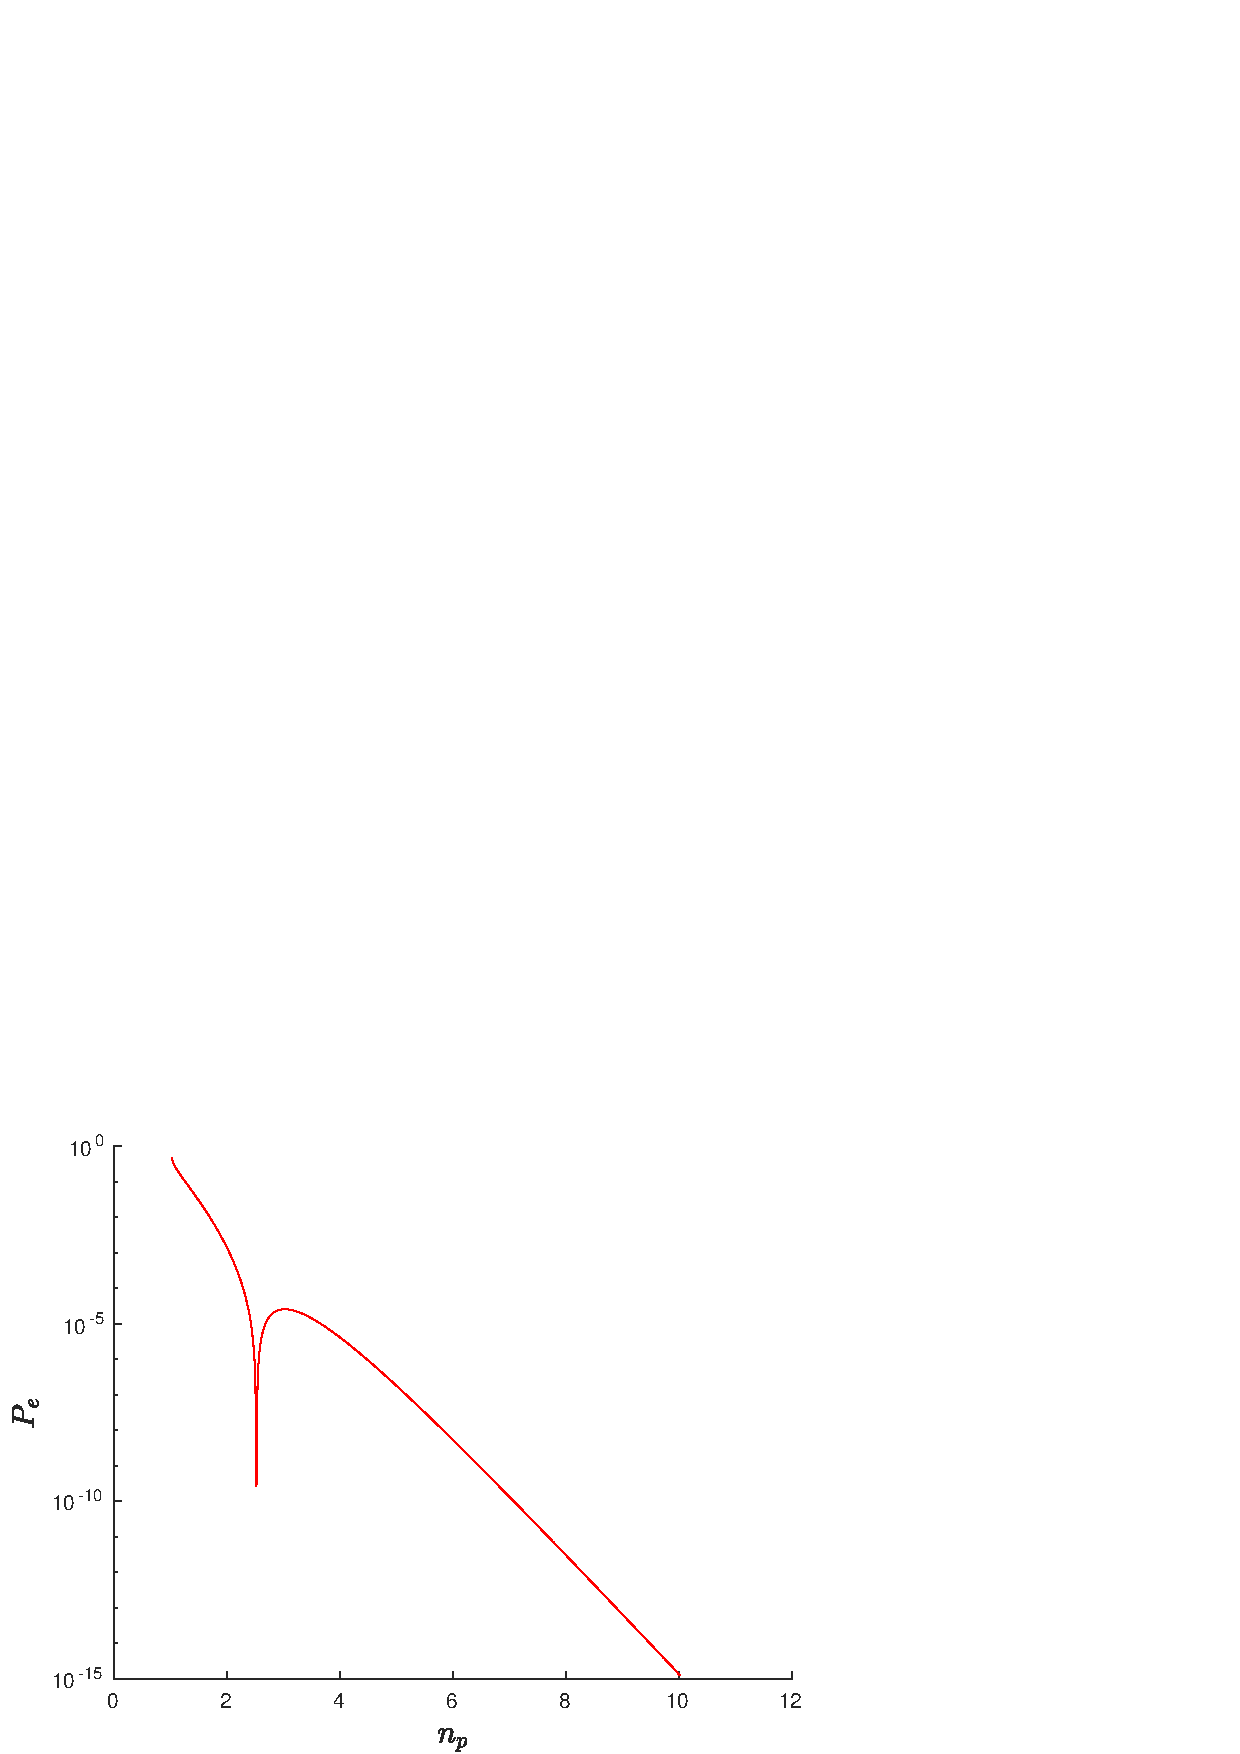
\includegraphics[width = 1\linewidth]{Pictures/fig3.2a.pdf}\\
                \scriptsize{
                    MDEP of a QBPSK with PACSs, without noise. $k=1$. 
                }
            \end{center}
        \end{column}
        \begin{column}{0.5\linewidth}
            \begin{center}
                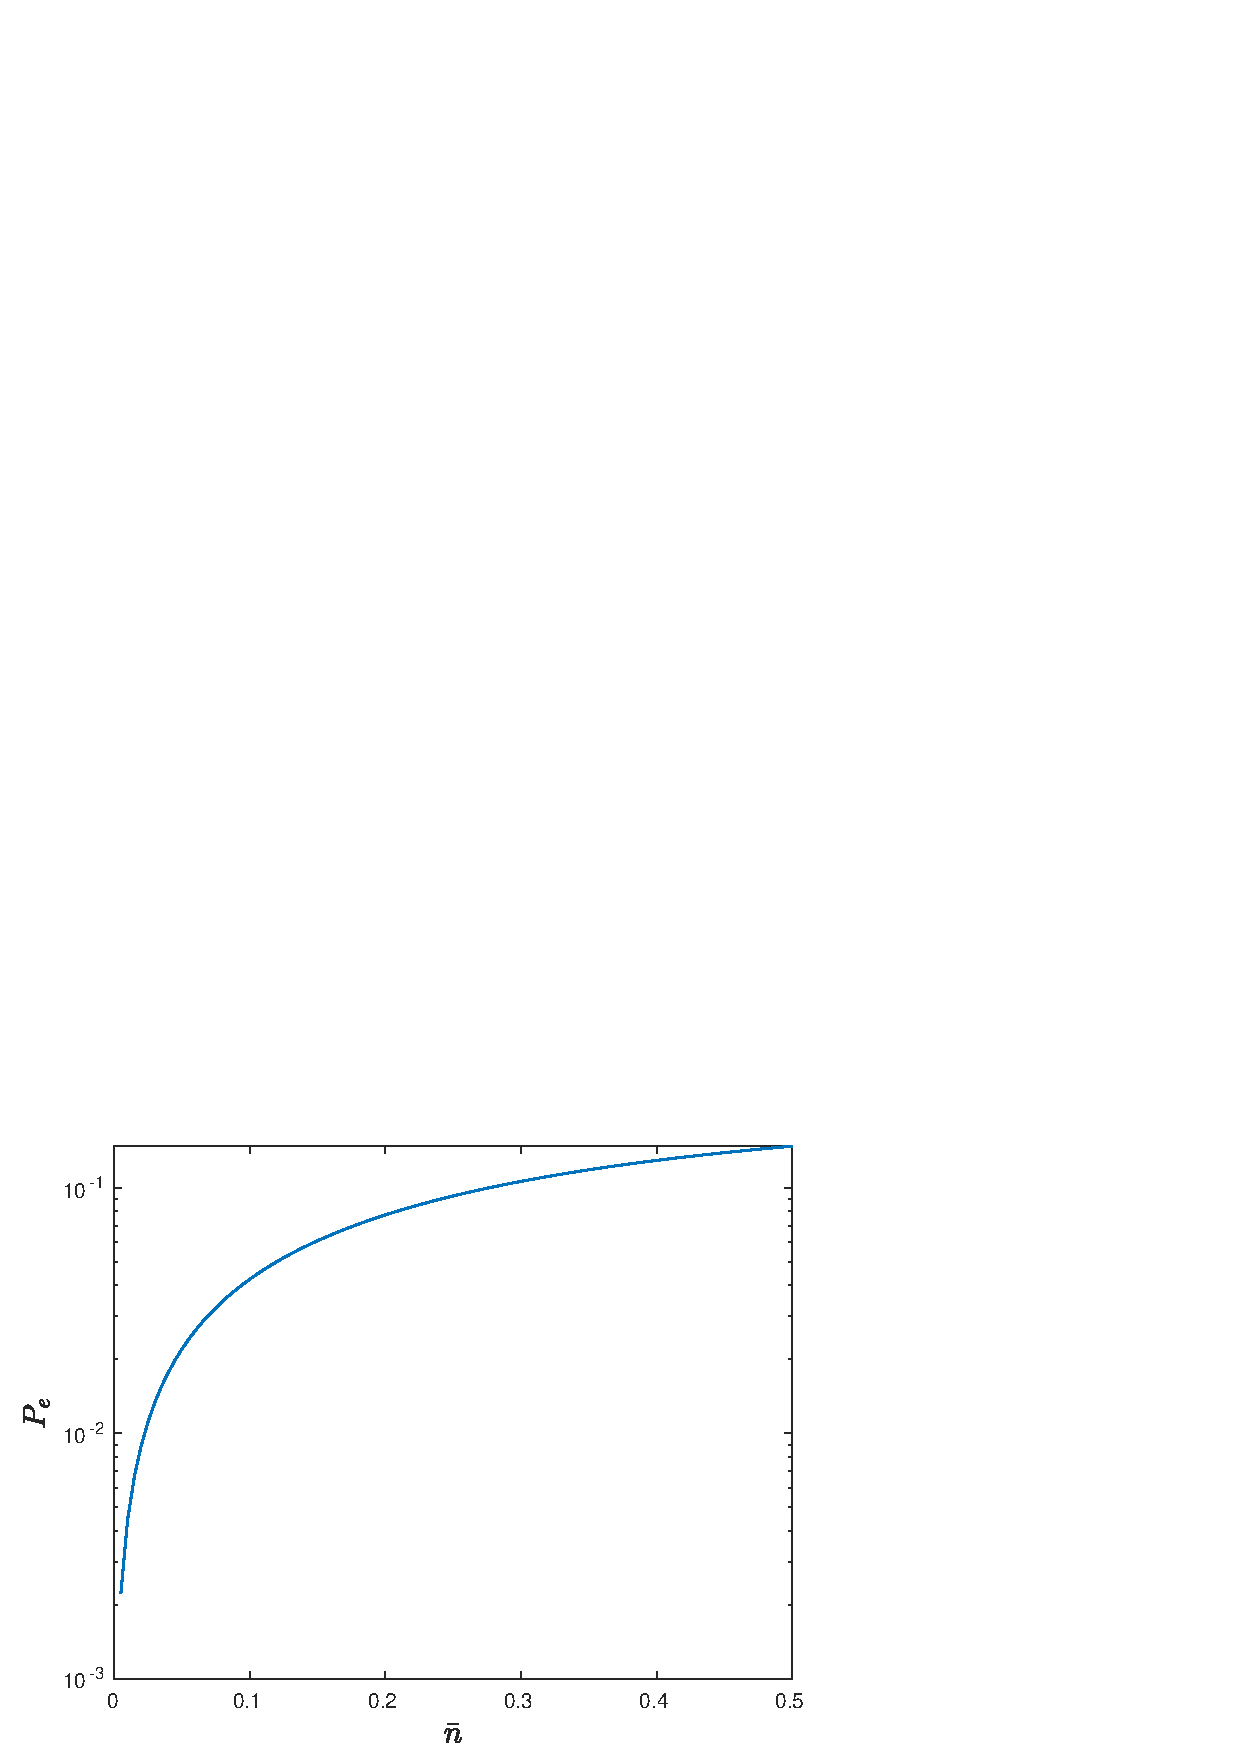
\includegraphics[width = 1\linewidth]{Pictures/fig3.3a.pdf}\\
                \scriptsize{
                    MDEP for $\mu=0.54$ (value of the zero) in terms of $\bar{n}$. 
                }
            \end{center}
        \end{column}
    \end{columns}
\end{frame}
    \subsection{Squeezed state system performance}
    \begin{frame}{Discrimination of Photon Added States}{Squeezed States discrimination: BPSK}
    \begin{center}
        \resizebox{0.7\textwidth}{!}{
            % This file was created by matlab2tikz.
%
%The latest updates can be retrieved from
%  http://www.mathworks.com/matlabcentral/fileexchange/22022-matlab2tikz-matlab2tikz
%where you can also make suggestions and rate matlab2tikz.
%
\definecolor{mycolor1}{rgb}{0.00000,0.44700,0.74100}%
\definecolor{mycolor2}{rgb}{0.85000,0.32500,0.09800}%
\definecolor{mycolor3}{rgb}{0.92900,0.69400,0.12500}%
\definecolor{mycolor4}{rgb}{0.49400,0.18400,0.55600}%
\definecolor{mycolor5}{rgb}{0.46600,0.67400,0.18800}%
%
\begin{tikzpicture}

\begin{axis}[%
width=4.602in*0.7,
height=3.617in*0.7,
at={(0.772in,0.488in)},
scale only axis,
unbounded coords=jump,
xmin=0,
xmax=6,
xlabel style={font=\color{white!15!black}},
xlabel={$\bar{n}_p$},
ymode=log,
ymin=1e-14,
ymax=1,
yminorticks=true,
ylabel style={font=\color{white!15!black}},
ylabel={$P_e$},
axis background/.style={fill=white},
axis x line*=bottom,
axis y line*=left,
legend style={at={(0,0)}, anchor=south west, legend cell align=left, align=left, draw=white!15!black}
]
\addplot [color=mycolor1, line width=1.0pt, mark=o, mark options={solid, mycolor1}, mark repeat={12}]
  table[row sep=crcr]{%
0	0.499389648066729\\
0.1	0.287120131656732\\
0.2	0.212910142400755\\
0.3	0.164146518823112\\
0.4	0.128963672155848\\
0.5	0.102469945641375\\
0.6	0.0820267587705491\\
0.7	0.0660057404300253\\
0.8	0.053316687804111\\
0.9	0.0431899288477864\\
1	0.035063149900423\\
1.1	0.0285136645710093\\
1.2	0.0232184417937623\\
1.3	0.0189265429755652\\
1.4	0.0154408902702601\\
1.5	0.0126055705880511\\
1.6	0.0102964976303587\\
1.7	0.00841409196053833\\
1.8	0.00687820690358171\\
1.9	0.00562430383176904\\
2	0.00460002577467994\\
2.1	0.00376302527499006\\
2.2	0.00307877636658277\\
2.3	0.00251928311932625\\
2.4	0.00206166744381331\\
2.5	0.00168731550747597\\
2.6	0.00138103408978052\\
2.7	0.00113041349779941\\
2.8	0.000925312013532187\\
2.9	0.0007574554395825\\
3	0.000620065121340496\\
3.1	0.000507610947614257\\
3.2	0.00041555845577157\\
3.3	0.00034020432004489\\
3.4	0.000278518326188193\\
3.5	0.000228019526022194\\
3.6	0.000186678411862207\\
3.7	0.000152834479756447\\
3.8	0.000125126403069165\\
3.9	0.000102442525523938\\
4	8.38712136650432e-05\\
4.1	6.86669296633413e-05\\
4.2	5.62189325594709e-05\\
4.3	4.60277414479071e-05\\
4.4	3.76841357328517e-05\\
4.5	3.08529664655999e-05\\
4.6	2.5260010464212e-05\\
4.7	2.06811547977526e-05\\
4.8	1.69321804356359e-05\\
4.9	1.38628034142552e-05\\
5	1.13498780289767e-05\\
5.1	9.29245618480623e-06\\
5.2	7.60801814436718e-06\\
5.3	6.22891236168321e-06\\
5.4	5.09979462653964e-06\\
5.5	4.17534106122996e-06\\
5.6	3.41849455004484e-06\\
5.7	2.79882051701374e-06\\
5.8	2.291476411731e-06\\
5.9	1.87610911872582e-06\\
6	1.53602182534351e-06\\
};
\addlegendentry{r = 0}

\addplot [color=mycolor2, line width=1.0pt, mark=square, mark options={solid, mycolor2}, mark repeat={12}]
  table[row sep=crcr]{%
0	nan\\
0.1	0.285384730399874\\
0.2	0.210689427589639\\
0.3	0.161777909175322\\
0.4	0.126605591806441\\
0.5	0.100209555121272\\
0.6	0.0799110816214625\\
0.7	0.0640579392955963\\
0.8	0.0515456333045833\\
0.9	0.0415956163871193\\
1	0.0336388963703997\\
1.1	0.0272500755834632\\
1.2	0.0221034685358382\\
1.3	0.0179476223469574\\
1.4	0.0145850823056448\\
1.5	0.0118603292716668\\
1.6	0.00964964889410247\\
1.7	0.00785436609664353\\
1.8	0.00639528103065568\\
1.9	0.00520869659653456\\
2	0.00424318733661139\\
2.1	0.00345728267523659\\
2.2	0.0028173621733017\\
2.3	0.00229616576838299\\
2.4	0.00187156088565621\\
2.5	0.00152560869850882\\
2.6	0.0012436658424142\\
2.7	0.00101389304306304\\
2.8	0.000826603033357909\\
2.9	0.000673935936456371\\
3	0.00054947811307765\\
3.1	0.000448014515359918\\
3.2	0.000365294341859612\\
3.3	0.000297851370744007\\
3.4	0.000242863287014505\\
3.5	0.000198028575768117\\
3.6	0.000161473027965209\\
3.7	0.000131666140895381\\
3.8	0.000107361399509842\\
3.9	8.75438435886666e-05\\
4	7.13850170852015e-05\\
4.1	5.82086286475825e-05\\
4.2	4.74643647291328e-05\\
4.3	3.87034684476983e-05\\
4.4	3.15597642202015e-05\\
4.5	2.57347559318166e-05\\
4.6	2.09846265820657e-05\\
4.7	1.71114586580146e-05\\
4.8	1.39531648718494e-05\\
4.9	1.13778034773748e-05\\
5	9.27775123749086e-06\\
5.1	7.56535751966769e-06\\
5.2	6.16899561722839e-06\\
5.3	5.03039927379767e-06\\
5.4	4.10191566646567e-06\\
5.5	3.34482333114172e-06\\
5.6	2.72746895979559e-06\\
5.7	2.22406304256628e-06\\
5.8	1.81355586392762e-06\\
5.9	1.47882610490591e-06\\
6	1.20587801633043e-06\\
};
\addlegendentry{r = 0.01}

\addplot [color=mycolor3, line width=1.0pt, mark=triangle, mark options={solid, mycolor3}, mark repeat={12}]
  table[row sep=crcr]{%
0	nan\\
0.1	0.289415146931883\\
0.2	0.201809855857211\\
0.3	0.148106262647244\\
0.4	0.11118917016601\\
0.5	0.0845566710160374\\
0.6	0.0648340163359155\\
0.7	0.0499886268732048\\
0.8	0.0386945489671331\\
0.9	0.0300377495744575\\
1	0.0233669723002363\\
1.1	0.01820634631197\\
1.2	0.0142024968506945\\
1.3	0.0110893558546985\\
1.4	0.00866470218395488\\
1.5	0.0067738503066016\\
1.6	0.00529786467496535\\
1.7	0.00414485651245422\\
1.8	0.00324358024638571\\
1.9	0.00253880918622246\\
2	0.00198746019863888\\
2.1	0.00155603923632802\\
2.2	0.00121838623270371\\
2.3	0.00095407210277898\\
2.4	0.000747140589099193\\
2.5	0.000585116528818652\\
2.6	0.000458242493606376\\
2.7	0.000358891396311511\\
2.8	0.000281085980332163\\
2.9	0.000220153339887175\\
3	0.000172430426453762\\
3.1	0.000135054099361875\\
3.2	0.00010578048178439\\
3.3	8.28524747186754e-05\\
3.4	6.48947335166739e-05\\
3.5	5.08288652040778e-05\\
3.6	3.98121878574242e-05\\
3.7	3.1183355076847e-05\\
3.8	2.4424723781058e-05\\
3.9	1.91310280652779e-05\\
4	1.49846616059879e-05\\
4.1	1.17370074078638e-05\\
4.2	9.19315691949585e-06\\
4.3	7.20071215398743e-06\\
4.4	5.6400946589763e-06\\
4.5	4.41768986703117e-06\\
4.6	3.4602287340979e-06\\
4.7	2.71029075338269e-06\\
4.8	2.12288811629602e-06\\
4.9	1.66278115582008e-06\\
5	1.30240617013389e-06\\
5.1	1.02012686953312e-06\\
5.2	7.99034826803879e-07\\
5.3	6.25856568348127e-07\\
5.4	4.90214389026189e-07\\
5.5	3.83971145101469e-07\\
5.6	3.00750263027005e-07\\
5.7	2.35568666906438e-07\\
5.8	1.84513678225251e-07\\
5.9	1.44523230938276e-07\\
6	1.13200048557083e-07\\
};
\addlegendentry{r = 0.1}

\addplot [color=mycolor4, line width=1.0pt, mark=diamond, mark options={solid, mycolor4}, mark repeat={12}]
  table[row sep=crcr]{%
0	nan\\
0.1	0.382834761043565\\
0.2	0.226726599948946\\
0.3	0.153725392982918\\
0.4	0.108252050696438\\
0.5	0.0776620274751858\\
0.6	0.0563246458453091\\
0.7	0.0411325196529638\\
0.8	0.0301767071385362\\
0.9	0.0222096066402786\\
1	0.0163825305797381\\
1.1	0.0121036873556075\\
1.2	0.00895283454360607\\
1.3	0.00662771889876096\\
1.4	0.00490945741015492\\
1.5	0.00363831365399447\\
1.6	0.00269719685540093\\
1.7	0.00200000212067292\\
1.8	0.00148329765169325\\
1.9	0.00110023686947414\\
2	0.000816170450806231\\
2.1	0.000605496164763131\\
2.2	0.000449227865912727\\
2.3	0.000333302734837115\\
2.4	0.000247298374210336\\
2.5	0.000183491253958834\\
2.6	0.000136149947847053\\
2.7	0.000101023902051689\\
2.8	7.49608315434025e-05\\
2.9	5.56222137316209e-05\\
3	4.12728773608873e-05\\
3.1	3.06252269954288e-05\\
3.2	2.27246137002313e-05\\
3.3	1.6862271223328e-05\\
3.4	1.25123100351843e-05\\
3.5	9.28446395787041e-06\\
3.6	6.88936954806874e-06\\
3.7	5.11211674480982e-06\\
3.8	3.79334780531426e-06\\
3.9	2.81476423491522e-06\\
4	2.08864027689826e-06\\
4.1	1.54982886191313e-06\\
4.2	1.15002554590404e-06\\
4.3	8.53350604679282e-07\\
4.4	6.33214201239962e-07\\
4.5	4.69863400409665e-07\\
4.6	3.48654844550822e-07\\
4.7	2.58711756129237e-07\\
4.8	1.91971829210935e-07\\
4.9	1.42448246642779e-07\\
5	1.05701118191526e-07\\
5.1	7.84336825487841e-08\\
5.2	5.82004880955722e-08\\
5.3	4.31862153815743e-08\\
5.4	3.20456979285844e-08\\
5.5	2.37788204127121e-08\\
5.6	1.76445323352148e-08\\
5.7	1.3092757544797e-08\\
5.8	9.71524360959819e-09\\
5.9	7.20903126083527e-09\\
6	5.34931965390228e-09\\
};
\addlegendentry{r = 0.2}

\addplot [color=mycolor5, line width=1.0pt, mark=x, mark options={solid, mycolor5}, mark repeat={12}]
  table[row sep=crcr]{%
0	nan\\
0.1	nan\\
0.2	nan\\
0.3	nan\\
0.4	nan\\
0.5	nan\\
0.6	0.242052787940402\\
0.7	0.121216545286974\\
0.8	0.0662369638239285\\
0.9	0.0373027657806079\\
1	0.0213046692452243\\
1.1	0.0122565814426305\\
1.2	0.00707933535974986\\
1.3	0.00409807822050423\\
1.4	0.00237533309698207\\
1.5	0.00137781245040047\\
1.6	0.000799513543964347\\
1.7	0.000464064935488784\\
1.8	0.00026938921586922\\
1.9	0.000156398005746461\\
2	9.08021041560736e-05\\
2.1	5.27190464215122e-05\\
2.2	3.06092537989966e-05\\
2.3	1.77722023697036e-05\\
2.4	1.03187613321176e-05\\
2.5	5.99128319045406e-06\\
2.6	3.47865527450253e-06\\
2.7	2.0197741404937e-06\\
2.8	1.17273831773401e-06\\
2.9	6.80913783190906e-07\\
3	3.95350652271365e-07\\
3.1	2.29549211083757e-07\\
3.2	1.33281825298592e-07\\
3.3	7.73865224124037e-08\\
3.4	4.49323004358959e-08\\
3.5	2.60884999714328e-08\\
3.6	1.51475686993585e-08\\
3.7	8.79500505757136e-09\\
3.8	5.10657599539499e-09\\
3.9	2.96500513030651e-09\\
4	1.72151681798738e-09\\
4.1	9.9955732579815e-10\\
4.2	5.803668101656e-10\\
4.3	3.3696778700687e-10\\
4.4	1.95653160339759e-10\\
4.5	1.13600739926056e-10\\
4.6	6.59591270490978e-11\\
4.7	3.82978093682595e-11\\
4.8	2.22364349156123e-11\\
4.9	1.29110611091221e-11\\
5	7.49589279536167e-12\\
5.1	4.35274039034539e-12\\
5.2	2.52714515980301e-12\\
5.3	1.46704870473968e-12\\
5.4	8.51874126794883e-13\\
5.5	4.94493335168045e-13\\
5.6	2.86992651865603e-13\\
5.7	1.66644475996236e-13\\
5.8	9.68114477473137e-14\\
5.9	5.61217738948017e-14\\
6	3.26405569239796e-14\\
};
\addlegendentry{r = 0.5}

\end{axis}
\end{tikzpicture}%
        }\\
        \scriptsize{
        MDEP of a QBPSK system with squeezed states in terms of the mean photon number in the system $\bar{n}_p$.\\
        $N=30$; $\bar{n}=0$; $p_0=p_1=1/2$
        }
    \end{center}

\end{frame}
    \subsection{PASS system performance}
    \begin{frame}{Discrimination of Photon Added States}{Noisy PASS discrimination}
    \center{\scriptsize $N=45$; $\bar{n}=10^{-2}$; $\theta=\pi$; $p_0=p_1=1/2$}
    \begin{columns}
        \begin{column}{0.5\linewidth}%<1->
            \begin{center}
                \resizebox{1\textwidth}{!}{
                    % This file was created by matlab2tikz.
%
%The latest updates can be retrieved from
%  http://www.mathworks.com/matlabcentral/fileexchange/22022-matlab2tikz-matlab2tikz
%where you can also make suggestions and rate matlab2tikz.
%
\definecolor{mycolor1}{rgb}{0.00000,0.44706,0.74118}%
\definecolor{mycolor2}{rgb}{0.85098,0.32549,0.09804}%
\definecolor{mycolor3}{rgb}{0.85098,0.32941,0.10196}%
\definecolor{mycolor4}{rgb}{0.92941,0.69020,0.12941}%
\definecolor{mycolor5}{rgb}{0.49412,0.18431,0.55686}%
\definecolor{mycolor6}{rgb}{0.49020,0.18039,0.56078}%
\definecolor{mycolor7}{rgb}{0.46667,0.67451,0.18824}%
%
\begin{tikzpicture}

\begin{axis}[%
width=4.521in,
height=3.566in,
at={(0.758in,0.481in)},
scale only axis,
xmin=0,
xmax=4,
xlabel style={font=\color{white!15!black}},
xlabel={$\bar{n}_p$},
ymode=log,
ymin=1e-07,
ymax=1,
yminorticks=true,
ylabel style={font=\color{white!15!black}},
ylabel={$P_e$},
axis background/.style={fill=white},
axis x line*=bottom,
axis y line*=left,
legend style={at={(0.151,0.133)}, anchor=south west, legend cell align=left, align=left, draw=white!15!black}
]
\addplot [color=mycolor1, dashed, line width=1.0pt]
  table[row sep=crcr]{%
0.0100000000010203	0.5\\
0.0100000000005099	0.451090572691058\\
0.0250000000005101	0.402886691283792\\
0.0500000000005101	0.356065452094155\\
0.08500000000051	0.311248795396144\\
0.13000000000051	0.268980151318818\\
0.18500000000051	0.229705791588748\\
0.25000000000051	0.193761885698297\\
0.32500000000051	0.161367836859558\\
0.41000000000051	0.132626017381623\\
0.50500000000051	0.107527572164159\\
0.61000000000051	0.0859635483991091\\
0.72500000000051	0.0677402706067526\\
0.850000000000511	0.0525976380078704\\
0.98500000000051	0.0402288938163128\\
1.13000000000051	0.030300412747497\\
1.28500000000051	0.0224701735043473\\
1.45000000000051	0.0164038154402497\\
1.62500000000051	0.0117874985937506\\
1.81000000000051	0.00833715723539569\\
2.00500000000051	0.00580411358757593\\
2.21000000000051	0.00397735316445369\\
2.42500000000051	0.00268301603344667\\
2.65000000000051	0.00178180465531275\\
2.88500000000051	0.00116504474732931\\
3.13000000000051	0.000750076554437373\\
3.38500000000051	0.000475529564681665\\
3.65000000000051	0.000296878649024612\\
3.92500000000051	0.000182524960914532\\
};
\addlegendentry{r = 0 \& k = 0}

\addplot [color=mycolor1, line width=1.0pt]
  table[row sep=crcr]{%
1.02000000000307	0.00495049504950945\\
0.519950970393687	0.00495049504951145\\
0.549238056382468	0.00495049384760837\\
0.596318098365133	0.00494513949975245\\
0.659059689574124	0.00485212464085472\\
0.735198210318913	0.00459825907392819\\
0.822700461899245	0.00420399327465371\\
0.919966333468088	0.00369559902026673\\
1.02587839224384	0.00312976798911424\\
1.13975229329811	0.00256690084404709\\
1.26124327363325	0.00204996332234814\\
1.39024719180321	0.00160098998755381\\
1.52681572702182	0.00122639811266967\\
1.67109195414956	0.000923250889520943\\
1.8232653201361	0.000683888328226578\\
1.98354224079897	0.000498830625317581\\
2.15212812011347	0.000358440774981539\\
2.32921719287323	0.000253800056086939\\
2.51498745769556	0.000177110101371558\\
2.70959877008803	0.000121819045365512\\
2.91319279840464	8.25922216302066e-05\\
3.1258940040236	5.52004961243968e-05\\
3.34781112191599	3.63708050424849e-05\\
3.57903882606496	2.36261622261202e-05\\
3.81965939805169	1.51315705133603e-05\\
};
\addlegendentry{r = 0 \& k = 1}

\addplot [color=mycolor2, dashed, line width=1.0pt]
  table[row sep=crcr]{%
0.0101020034000452	0.496440221166252\\
0.0100510017000226	0.450685266879101\\
0.0250510017000227	0.402323848857672\\
0.0500510017000227	0.355323831951221\\
0.0850510017000227	0.310342569240449\\
0.130051001700023	0.267937053924156\\
0.185051001700023	0.228561577996887\\
0.250051001700023	0.192555962356324\\
0.325051001700022	0.160139898037218\\
0.410051001700022	0.131413390802683\\
0.505051001700022	0.106363150238377\\
0.610051001700022	0.084874304451924\\
0.725051001700022	0.0667463796210962\\
0.850051001700022	0.0517121945793499\\
0.985051001700022	0.0394581777272386\\
1.13005100170002	0.0296446106224665\\
1.28505100170002	0.0219244325201435\\
1.45005100170002	0.0159594874610171\\
1.62505100170002	0.0114334328178015\\
1.81005100170002	0.00806091588240215\\
2.00505100170002	0.00559301485214148\\
2.21005100170002	0.00381928293290495\\
2.42505100170002	0.00256698805700845\\
2.65005100170002	0.0016982819014697\\
2.88505100170002	0.00110605829688115\\
3.13005100170002	0.00070919103279321\\
3.38505100170003	0.000447706522481883\\
3.65005100170002	0.000278284092734504\\
3.92505100170002	0.000170317624234251\\
};
\addlegendentry{r = 0.01 \& k = 0}

\addplot [color=mycolor3, line width=1.0pt]
  table[row sep=crcr]{%
1.0203070200328	0.00495049504950934\\
0.520003993727059	0.00495049504785372\\
0.549001157710359	0.00495038332939279\\
0.595633295725975	0.0049392571443127\\
0.657812406575135	0.00482687502920459\\
0.733319931015453	0.0045631231538617\\
0.820163956671601	0.00416202053329034\\
0.916776798855965	0.00365102850298482\\
1.02206361072068	0.00308652722310032\\
1.13535382816234	0.002527430960577\\
1.25630958280929	0.00201533049463498\\
1.38482876156695	0.00157141039702463\\
1.52096193052793	0.00120164880320228\\
1.66484921648061	0.000902903844066383\\
1.81667619389296	0.000667431624103765\\
1.97664507461977	0.000485731323126737\\
2.14495708856206	0.000348179400141146\\
2.32180252953073	0.000245890780959823\\
2.50735578881924	0.000171112861362621\\
2.70177348530881	0.00011734628488913\\
2.90519442114697	7.93115435048231e-05\\
3.11774054123651	5.28340238664105e-05\\
3.33951838323524	3.46919847475369e-05\\
3.57062070885033	2.24547493862248e-05\\
3.81112813837093	1.43275426212064e-05\\
};
\addlegendentry{r = 0.01 \& k = 1}

\addplot [color=mycolor4, dashed, line width=1.0pt]
  table[row sep=crcr]{%
0.0202340453657284	0.464473627654879\\
0.0151170226828645	0.437604627349995\\
0.0301170226828643	0.392232608937378\\
0.0551170226828643	0.345350311735397\\
0.0901170226828644	0.299872457829165\\
0.135117022682864	0.256926510392587\\
0.190117022682864	0.217172327050335\\
0.255117022682864	0.181031813929761\\
0.330117022682864	0.148752335319914\\
0.415117022682864	0.120429087835948\\
0.510117022682864	0.0960200366887284\\
0.615117022682864	0.0753645347394633\\
0.730117022682865	0.0582063945825236\\
0.855117022682864	0.0442194749392917\\
0.990117022682864	0.033033747624904\\
1.13511702268286	0.0242600166699049\\
1.29011702268286	0.0175117313604393\\
1.45511702268286	0.012422724228866\\
1.63011702268287	0.0086601979591992\\
1.81511702268287	0.00593281764231124\\
2.01011702268286	0.00399425837705447\\
2.21511702268287	0.00264294241797458\\
2.43011702268287	0.00171892901031734\\
2.65511702268286	0.00109898195775715\\
2.89011702268287	0.000690756906602363\\
3.13511702268287	0.000426868293537996\\
3.39011702268287	0.000259369510946184\\
3.65511702268287	0.000154957633989594\\
3.93011702268287	9.10290546821124e-05\\
};
\addlegendentry{r = 0.1 \& k = 0}

\addplot [color=mycolor4, line width=1.0pt]
  table[row sep=crcr]{%
1.05080244685835	0.00494855515487186\\
0.534305855441027	0.00493956193944328\\
0.560577815242343	0.00489125057574918\\
0.603010711176586	0.00476554057726364\\
0.659935286045382	0.00454063398198279\\
0.729573342297954	0.00420193412015313\\
0.810323033235768	0.00375582941028574\\
0.90091844851316	0.0032368659457353\\
1.00047082343265	0.00269516501446371\\
1.10843171757119	0.00217671120450486\\
1.22452096613732	0.00171213398444298\\
1.3486495574248	0.00131595523776701\\
1.4808530565899	0.00099074984674008\\
1.62124071752346	0.000731856527585784\\
1.76995971625628	0.000531006006724011\\
1.92717165481784	0.000378693077575321\\
2.09303809416422	0.000265572059704344\\
2.26771230591607	0.000183193116200464\\
2.45133509281032	0.000124323441114904\\
2.64403315014596	8.30191324586171e-05\\
2.8459189361002	5.45554227568412e-05\\
3.05709138017673	3.5284096614796e-05\\
3.27763700858953	2.24616790437393e-05\\
3.50763123129931	1.40753992720621e-05\\
3.74713964255157	8.68275836485299e-06\\
3.99621925419453	5.27284023565944e-06\\
};
\addlegendentry{r = 0.1 \& k = 1}

\addplot [color=mycolor5, dashed, line width=1.0pt]
  table[row sep=crcr]{%
0.051346909637612	0.429393647208632\\
0.0306734548188061	0.411688903318411\\
0.045673454818806	0.373223243143298\\
0.070673454818806	0.329064496412081\\
0.105673454818806	0.284699966244283\\
0.150673454818806	0.242312311121901\\
0.205673454818806	0.20300894013495\\
0.270673454818806	0.167412745153845\\
0.345673454818806	0.135848539010154\\
0.430673454818806	0.108424113178776\\
0.525673454818806	0.085074901679797\\
0.630673454818806	0.0655975019569672\\
0.745673454818806	0.0496824127447445\\
0.870673454818806	0.0369476450892914\\
1.00567345481881	0.0269714468453113\\
1.15067345481881	0.0193219002119312\\
1.30567345481881	0.0135816008581836\\
1.47067345481881	0.00936630014651907\\
1.64567345481881	0.00633712474233589\\
1.83067345481881	0.00420668870569196\\
2.02567345481881	0.00273998478983489\\
2.23067345481881	0.00175130670345874\\
2.44567345481881	0.00109858125431284\\
2.67067345481881	0.000676400651179798\\
2.90567345481881	0.000408804118392059\\
3.15067345481881	0.000242545209768685\\
3.40567345481881	0.000141270680246663\\
3.67067345481881	8.07790992743973e-05\\
3.94567345481881	4.53451833415941e-05\\
};
\addlegendentry{r = 0.2 \& k = 0}

\addplot [color=mycolor6, line width=1.0pt]
  table[row sep=crcr]{%
1.14443400452204	0.00479106599394818\\
0.579999501304023	0.00475077465542328\\
0.603041046327231	0.00463108156969505\\
0.640504199710634	0.00442827805532442\\
0.691224117225214	0.00413258381262105\\
0.753950466998375	0.00374355433932783\\
0.827545812383434	0.00327986823785392\\
0.911100241882687	0.00277718849843345\\
1.00396497754985	0.00227642511237597\\
1.10573089526536	0.0018115455221398\\
1.21618079241689	0.00140378131439783\\
1.33523645804668	0.0010619876604348\\
1.46291195118471	0.000785891546957074\\
1.5992772335824	0.000569691758631641\\
1.7444321745409	0.000404922413376918\\
1.89848917670023	0.000282385374672289\\
2.06156226583414	0.0001933054291125\\
2.23376070757581	0.000129931168492581\\
2.41518563437222	8.57733261649951e-05\\
2.60592858523409	5.56215786678416e-05\\
2.80607120496685	3.54369671975441e-05\\
3.01568560586141	2.21846003883308e-05\\
3.23483507482365	1.36482495925461e-05\\
3.46357493039391	8.25216498795411e-06\\
3.70195341365423	4.90393868035621e-06\\
3.9500125478046	2.86426889811731e-06\\
};
\addlegendentry{r = 0.2 \& k = 1}

\addplot [color=mycolor7, dashed, line width=1.0pt]
  table[row sep=crcr]{%
0.286971123755774	0.330768077356153\\
0.148485561877887	0.321870897864741\\
0.163485561877887	0.2980861532608\\
0.188485561877887	0.265400945113278\\
0.223485561877887	0.229097440353421\\
0.268485561877887	0.192694408147652\\
0.323485561877887	0.158325364694675\\
0.388485561877887	0.127217381024676\\
0.463485561877887	0.0999991591056063\\
0.548485561877887	0.0768883603237902\\
0.643485561877887	0.0578110254090491\\
0.748485561877886	0.042489385074143\\
0.863485561877887	0.0305142243008485\\
0.988485561877887	0.0214056829491879\\
1.12348556187789	0.0146637973864988\\
1.26848556187789	0.0098079816862493\\
1.42348556187789	0.00640463929230534\\
1.58848556187789	0.00408314565752849\\
1.76348556187788	0.00254163692367282\\
1.94848556187788	0.00154491239086835\\
2.14348556187788	0.000917124936882341\\
2.34848556187788	0.000531801834133649\\
2.56348556187788	0.000301247165333363\\
2.78848556187787	0.000166721564607453\\
3.02348556187786	9.01545309603957e-05\\
3.26848556187785	4.76353769972571e-05\\
3.52348556187783	2.45938563666614e-05\\
3.78848556187779	1.24073309797912e-05\\
};
\addlegendentry{r = 0.5 \& k = 0}

\addplot [color=mycolor7, line width=1.0pt]
  table[row sep=crcr]{%
1.85306548733767	0.00353641115520514\\
0.930796962701587	0.00348196426464287\\
0.943656157582369	0.00332231969133245\\
0.965295445105895	0.00306951882024781\\
0.995980641808412	0.00274452597887531\\
1.03601054788413	0.00237451347003192\\
1.08567365297189	0.0019883961081173\\
1.14521827738196	0.00161265536534688\\
1.21483826418498	0.00126811447852393\\
1.29467137765998	0.000968122366654389\\
1.38480564628563	0.000718538771233457\\
1.48528924260403	0.000519112688197765\\
1.59614083486364	0.000365447596944291\\
1.71735873922715	0.000250906556350627\\
1.84892823171401	0.000168117888699859\\
1.9908269892895	0.000109991365809137\\
2.14302891711736	7.02953013373975e-05\\
2.30550670737067	4.38998630067355e-05\\
2.47823346100084	2.67972348785284e-05\\
2.66118364860192	1.59921449159883e-05\\
2.85433362280369	9.33241343792357e-06\\
3.05766183728397	5.32614461246084e-06\\
3.27114888140597	2.97307164354166e-06\\
3.49477740479924	1.62328253511257e-06\\
3.7285319812022	8.66931754384126e-07\\
3.97239894341011	4.5286496330732e-07\\
};
\addlegendentry{r = 0.5 \& k = 1}

\end{axis}

\begin{axis}[%
width=5.833in,
height=4.375in,
at={(0in,0in)},
scale only axis,
xmin=0,
xmax=1,
ymin=0,
ymax=1,
axis line style={draw=none},
ticks=none,
axis x line*=bottom,
axis y line*=left
]
\end{axis}
\end{tikzpicture}%
                }\\
                \scriptsize{
                MDEP of a QOOK system with PASS in terms of the mean photon number in the system $\bar{n}_p$.\\
                }
            \end{center}
        %\end{frame}
        \end{column}
        
        \begin{column}{0.5\linewidth}%<2->
            %\begin{frame}{Discrimination of Photon Added States}{Noisy PASS discrimination: BPSK}
            \begin{center}
                \resizebox{1\textwidth}{!}{
                    % This file was created by matlab2tikz.
%
%The latest updates can be retrieved from
%  http://www.mathworks.com/matlabcentral/fileexchange/22022-matlab2tikz-matlab2tikz
%where you can also make suggestions and rate matlab2tikz.
%
\definecolor{mycolor1}{rgb}{0.00000,0.44706,0.74118}%
\definecolor{mycolor2}{rgb}{0.85098,0.32941,0.10196}%
\definecolor{mycolor3}{rgb}{0.85098,0.32549,0.09804}%
\definecolor{mycolor4}{rgb}{0.92941,0.69020,0.12941}%
\definecolor{mycolor5}{rgb}{0.92941,0.69412,0.12549}%
\definecolor{mycolor6}{rgb}{0.49020,0.18039,0.56078}%
\definecolor{mycolor7}{rgb}{0.49412,0.18431,0.55686}%
\definecolor{mycolor8}{rgb}{0.47059,0.67059,0.18824}%
\definecolor{mycolor9}{rgb}{0.46667,0.67451,0.18824}%
%
\begin{tikzpicture}

\begin{axis}[%
width=4.521in,
height=3.566in,
at={(0.758in,0.481in)},
scale only axis,
xmin=0,
xmax=10,
xlabel style={font=\color{white!15!black}},
xlabel={$\bar{n}_p$},
ymode=log,
ymin=1.11022302462516e-16,
ymax=1,
yminorticks=true,
ylabel style={font=\color{white!15!black}},
ylabel={$P_e$},
axis background/.style={fill=white},
axis x line*=bottom,
axis y line*=left,
legend style={at={(0.172,0.138)}, anchor=south west, legend cell align=left, align=left, draw=white!15!black}
]
\addplot [color=mycolor1, dashed, line width=1.0pt]
  table[row sep=crcr]{%
0.0200000000020406	0.5\\
0.0400000000020402	0.402886691283791\\
0.10000000000204	0.311248795396143\\
0.20000000000204	0.229705791588748\\
0.34000000000204	0.161367836859558\\
0.52000000000204	0.107527572164159\\
0.740000000002041	0.0677402706067528\\
1.00000000000204	0.040228893816313\\
1.30000000000204	0.0224701735043469\\
1.64000000000204	0.0117874985937501\\
2.02000000000204	0.00580411358757571\\
2.44000000000204	0.00268301603344689\\
2.90000000000204	0.00116504474732904\\
3.40000000000204	0.000475529564681332\\
3.94000000000204	0.00018252496091431\\
4.52000000000204	6.58942320924671e-05\\
5.14000000000204	2.2372962739603e-05\\
5.80000000000205	7.14262612222516e-06\\
6.50000000000204	2.14348977123358e-06\\
7.24000000000202	6.04459258424228e-07\\
8.02000000000186	1.60120172343348e-07\\
8.84000000000037	3.98308174776041e-08\\
9.69999999998796	9.30169952173543e-09\\
};
\addlegendentry{r = 0 \& k = 0}

\addplot [color=mycolor1, line width=1.0pt]
  table[row sep=crcr]{%
2.04000000000614	0.5\\
2.07980388157475	0.365238945696499\\
2.19695222552987	0.245075031520992\\
2.38527239346053	0.149666545304717\\
2.6362387582965	0.0824178394910576\\
2.94079284127565	0.0405450261122263\\
3.29080184759698	0.0176651515033895\\
3.67986533387235	0.0067767120762533\\
4.10351356897534	0.00229560228979309\\
4.55900917319244	0.000707434570884347\\
5.04497309453299	0.00021948919726017\\
5.56098876721283	8.28582489130203e-05\\
6.10726290808727	4.1022391904566e-05\\
6.68436781659824	2.27142595118912e-05\\
7.29306128054439	1.21004232845334e-05\\
7.93416896319587	5.8707409222869e-06\\
8.60851248045389	2.56977332785402e-06\\
9.31686877149291	1.01844033345566e-06\\
};
\addlegendentry{r = 0 \& k = 1}

\addplot [color=mycolor2, dashed, line width=1.0pt]
  table[row sep=crcr]{%
0.0202040068000908	0.5\\
0.0402040068000913	0.401929857312568\\
0.10020400680009	0.309497261534983\\
0.200204006800091	0.227441434498448\\
0.34020400680009	0.158921613934891\\
0.520204006800091	0.105203426893547\\
0.74020400680009	0.0657565949389308\\
1.00020400680009	0.0386924167915099\\
1.30020400680009	0.02138427717136\\
1.64020400680009	0.0110847482118906\\
2.02020400680009	0.00538636930314729\\
2.44020400680009	0.00245418111590695\\
2.90020400680009	0.00104914081956387\\
3.40020400680009	0.000421078922301255\\
3.94020400680009	0.000158737723952473\\
4.52020400680009	5.62134664584546e-05\\
5.1402040068001	1.86983044717093e-05\\
5.80020400680009	5.84067384179487e-06\\
6.50020400680009	1.71271516641314e-06\\
7.24020400680009	4.71320126316233e-07\\
8.02020400680005	1.21675566899793e-07\\
8.84020400679961	2.94582267468257e-08\\
9.70020400679538	6.68653471480596e-09\\
};
\addlegendentry{r = 0.01 \& k = 0}

\addplot [color=mycolor3, line width=1.0pt]
  table[row sep=crcr]{%
2.04061404006561	0.5\\
2.08001597490824	0.363953791657615\\
2.19600463084144	0.242890205025005\\
2.3825331829039	0.147175347943858\\
2.63124962630054	0.0801720725339249\\
2.93327972406181	0.0388700383719509\\
3.28065582668641	0.016617401220776\\
3.66710719542386	0.00622702749712573\\
4.08825444288274	0.00205619367735721\\
4.54141531264937	0.000623306805922375\\
5.02523833123715	0.000197591171319678\\
5.5393150462678	8.00537851518568e-05\\
6.08384772211171	4.18763616073514e-05\\
6.65939686592245	2.33559660586802e-05\\
7.26670477557184	1.22187443445387e-05\\
7.90658029847907	5.77316485922408e-06\\
8.57982835424825	2.4554655915221e-06\\
9.28721011812292	9.45040670941033e-07\\
};
\addlegendentry{r = 0.01 \& k = 1}

\addplot [color=mycolor4, dashed, line width=1.0pt]
  table[row sep=crcr]{%
0.0404680907314567	0.5\\
0.0604680907314585	0.392901670542549\\
0.120468090731458	0.293128630573881\\
0.220468090731458	0.206620339442921\\
0.360468090731457	0.136941029534563\\
0.540468090731457	0.084941538631533\\
0.760468090731459	0.0491016108355734\\
1.02046809073146	0.026360899632598\\
1.32046809073146	0.0131130551179189\\
1.66046809073146	0.00603787611242568\\
2.04046809073146	0.00257369694341059\\
2.46046809073146	0.00101640450241469\\
2.92046809073146	0.000372205972558992\\
3.42046809073146	0.00012645461779881\\
3.96046809073146	3.98629468535416e-05\\
4.54046809073146	1.16575616797565e-05\\
5.16046809073146	3.16151968782208e-06\\
5.82046809073146	7.94771541634542e-07\\
6.52046809073146	1.85116668105501e-07\\
7.26046809073146	3.99314517562921e-08\\
8.04046809073146	7.97410959485489e-09\\
8.86046809073146	1.47367751335281e-09\\
9.72046809073146	2.51973775178271e-10\\
};
\addlegendentry{r = 0.1 \& k = 0}

\addplot [color=mycolor5, line width=1.0pt]
  table[row sep=crcr]{%
2.1016048937167	0.5\\
2.13722342176411	0.351557555027417\\
2.24231126096937	0.222160769918723\\
2.41204284470634	0.124222362453645\\
2.63974114418153	0.0603925042112791\\
2.91829336919182	0.0250484475022711\\
3.24129213294307	0.00872798119433771\\
3.60367379405264	0.00258598757293121\\
4.0018832937306	0.000741253402724129\\
4.43372687028477	0.000287093498001045\\
4.89808386454928	0.000162974574048513\\
5.39459822969919	9.8293093218349e-05\\
5.9234122263596	5.2962165794368e-05\\
6.48496287009384	2.48063685127087e-05\\
7.07983886502512	1.01844444848065e-05\\
7.70868661927138	3.70885692668743e-06\\
8.37215237665687	1.20946493997742e-06\\
9.07084922366429	3.55623495429391e-07\\
9.80534037124127	9.47534976036835e-08\\
};
\addlegendentry{r = 0.1 \& k = 1}

\addplot [color=mycolor6, dashed, line width=1.0pt]
  table[row sep=crcr]{%
0.102693819275224	0.5\\
0.122693819275224	0.381945077116474\\
0.182693819275225	0.273671210068553\\
0.282693819275225	0.18272455257\\
0.422693819275225	0.112952560216816\\
0.602693819275226	0.0642502792905548\\
0.822693819275224	0.03345396094764\\
1.08269381927522	0.0158838250522541\\
1.38269381927522	0.00686368066298626\\
1.72269381927522	0.00269897231763505\\
2.10269381927523	0.000966736234112642\\
2.52269381927523	0.000315777240763426\\
2.98269381927522	9.41232533182568e-05\\
3.48269381927522	2.56024275193667e-05\\
4.02269381927522	6.35315675889814e-06\\
4.60269381927523	1.43743867431212e-06\\
5.22269381927523	2.96354467355098e-07\\
5.88269381927523	5.5640574203597e-08\\
6.58269381927523	9.50809414534959e-09\\
7.32269381927523	1.47814516182621e-09\\
8.10269381927523	2.08976613791378e-10\\
8.92269381927523	2.68594035901515e-11\\
9.78269381927522	3.13798986795177e-12\\
};
\addlegendentry{r = 0.2 \& k = 0}

\addplot [color=mycolor7, line width=1.0pt]
  table[row sep=crcr]{%
2.28886800904409	0.5\\
2.31999800521609	0.335903697984307\\
2.41216418530892	0.196933331036258\\
2.56201679884254	0.0981076147304128\\
2.76489646890086	0.040185809256969\\
3.0158018679935	0.0130832203468926\\
3.31018324953374	0.00344887391962134\\
3.64440096753075	0.00101951363497232\\
4.01585991019939	0.000567040966715227\\
4.42292358106145	0.000392962039574174\\
4.86472316966757	0.000231481537813827\\
5.34094583218671	0.000111581978084918\\
5.85164780473884	4.51448958011524e-05\\
6.39710893432961	1.56946401249081e-05\\
6.97772869816361	4.76400489057838e-06\\
7.59395670680091	1.27574898745042e-06\\
8.24624906333657	3.03436716753147e-07\\
8.93504283030325	6.43988304904752e-08\\
9.66074253748888	1.2235391422255e-08\\
};
\addlegendentry{r = 0.2 \& k = 1}

\addplot [color=mycolor8, dashed, line width=1.0pt]
  table[row sep=crcr]{%
0.573942245572178	0.5\\
0.593942245028823	0.342499519674481\\
0.653942245170735	0.20790550335767\\
0.753942245341616	0.110057719920144\\
0.893942244583911	0.0500472584431716\\
1.07394224497389	0.0193143675146228\\
1.293942244546	0.00628332214973615\\
1.55394224371114	0.00172174882973891\\
1.85394224420503	0.000398395169961208\\
2.19394224278596	7.80046198984863e-05\\
2.57394224201761	1.29266966575337e-05\\
2.99394224220523	1.81130230003657e-06\\
3.45394223899107	2.14287482536157e-07\\
3.95394223844945	2.13728023612525e-08\\
4.49394223715584	1.79488168772224e-09\\
5.07394223021208	1.26788857190974e-10\\
5.693942230031	7.52714557350487e-12\\
6.35394222368679	3.74977826567147e-13\\
7.05394220748901	1.55431223447522e-14\\
7.79394220753813	4.44089209850063e-16\\
8.57394218450974	1.11022302462516e-16\\
9.39394214003978	0\\
};
\addlegendentry{r = 0.5 \& k = 0}

\addplot [color=mycolor9, line width=1.0pt]
  table[row sep=crcr]{%
3.7061308486222	0.5\\
3.72318775095693	0.276003723186423\\
3.77462452178882	0.111964236743116\\
3.86118165596315	0.0292098038693948\\
3.98392247081425	0.00541832505604978\\
4.14404207041508	0.00392337294658973\\
4.34269448841782	0.00386065139664005\\
4.58087300628471	0.00224591730584783\\
4.85935291484359	0.000870231139084243\\
5.17868537920139	0.000246879397142796\\
5.53922245734845	5.40728938508428e-05\\
5.94115678880561	9.42866109115981e-06\\
6.38456317979691	1.33219265713302e-06\\
6.86943477192184	1.54061789436888e-07\\
7.39571266351863	1.46675764867155e-08\\
7.96330772743687	1.15372272846415e-09\\
8.57211535637269	7.51390061282109e-11\\
9.22202638435226	4.05170341721828e-12\\
9.9129334474046	1.78523862359725e-13\\
};
\addlegendentry{r = 0.5 \& k = 1}

\end{axis}

\begin{axis}[%
width=5.833in,
height=4.375in,
at={(0in,0in)},
scale only axis,
xmin=0,
xmax=1,
ymin=0,
ymax=1,
axis line style={draw=none},
ticks=none,
axis x line*=bottom,
axis y line*=left
]
\end{axis}
\end{tikzpicture}%
                }\\
                \scriptsize{
                MDEP of a QBPSK system with PASS in terms of the mean photon number in the system $\bar{n}_p$.\\
                }
            \end{center}
        \end{column}
    \end{columns}
 \mbox{} \\ \mbox{} \\
\end{frame}  

    \section{Conclusion}
    % Conclusioni

\chapter{Conclusion}
    The aim of this thesis is analyzing the perfomance of a quantum optimal discriminator in the 
    presence of non-gaussian states. This perfomance was evaluated in terms of error probability 
    relating to symbol recognition. 
    In the first place, we have presented the quantum mechanics postulates, formulated by Dirac and 
    Von Neumann and generalized with the use of density operators.
    Then, we have described the quantum modulation and quantum states discrimination concepts. 
    Finally, we have analyzed some systems perfomance in terms of minimum distribution error 
    probability (MDEP).
    All evaluations were made assuming the absence of effects associated to the communication channel, 
    then supposing that the recieved state does not present any difference compared to the emitted one.
    
    This thesis highlights the fact that the use of non-gaussian photon added states instead of gaussian 
    states in OOK systems can ameliorate the QSD.
    In particular, the combination of squeezing and photon addition (PASSs) turns out extremely effective.
    Instead, in BPSK quantum systems, the photon addition effect manifests itself as negative.

    The obtained results can be significantly important in a quantum communication system design, 
    allowing us to make the best of this phisic theory potential. 
\end{document}